\documentclass[../00_Main.tex]{subfiles}
\begin{document}

Una de las funciones principales de este algoritmo es DrugSignal (\href{https://github.com/faturita/python-nerv/blob/master/DrugSignal.py}{drugsignal.py}), permite inyectar el erptemplate en las ubicaciones correctas basado en la información de t_flash. 

A medida que se recorren los vectores mencionados, se ejecuta una regresión logística con las métricas de  \textit{precision, recall y f1-score}, tanto para los hit como para los nohit, que son las marcas donde se identifica si hay o no un disparo de P300. 

El experimento se realizó con las cuatro señales correspondientes a los pacientes denominados pasivos, arrojando el mismo comportamiento en las modificaciones propuestas en este trabajo.

\subsection{Variaciones en amplitud.}
Se realizaron pruebas con distintos vectores de distintos tamaños, que generaron modificaciones en la amplitud del orden de los micro Voltios. \textbf{Para alteraciones en amplitud}, y tanto en disparos de hit como en nohit, existen intervalos en donde se mejoran los resultados y que el algoritmo se estabiliza aun cuando se pueda continuar realizando variaciones. Esto sucede porque la amplitud es una característica de la señal que, si bien puede aportar mejorías, los disparos de hit/nohit son fenómenos en la señal t-flash que suceden en el tiempo. 

La calidad del modelo, dada por la métrica de \textit{precision}, presenta mejorías cuando se varía la amplitud, pero se estanca cuando supera un umbral. La amplitud no afecta los resultados después de los 5 µV.

\begin{figure}[H]
    \raggedright
    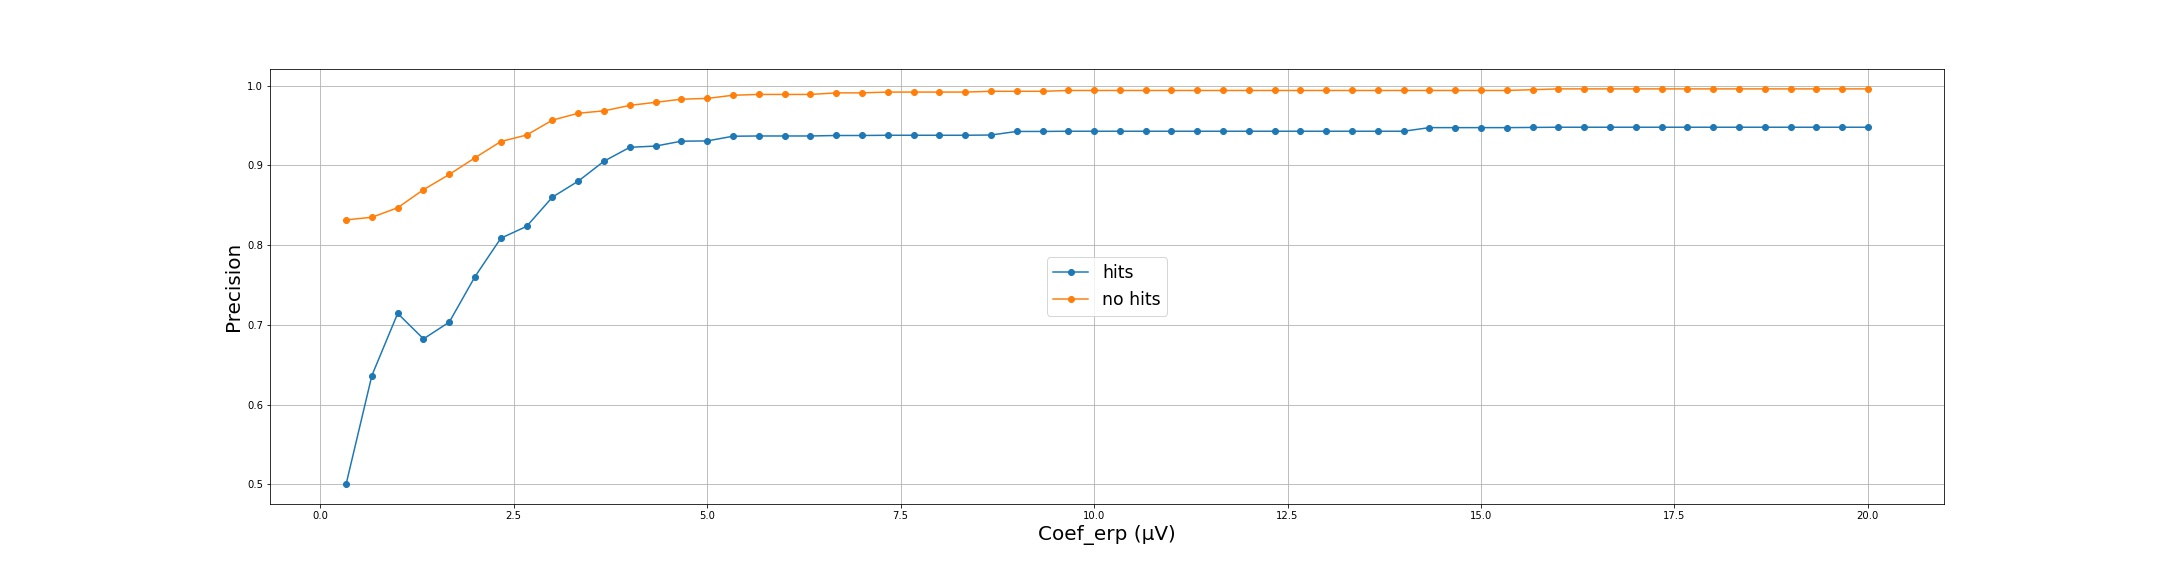
\includegraphics[scale=0.26]{02_Images/resultados_caso1_a_precision}
    \caption{Variación en uV para detectar el rendimiento en función de la métrica Precisión..}
    \label{fig:resultados_caso1_a_precision}
\end{figure}  

La proporción de resultados positivos que fueron identificados como tal, también presenta el mismo comportamiento  que la \textit{recall}, dando mejorías hasta los 5 µV para luego estancarse.

\begin{figure}[H]
    \raggedright
    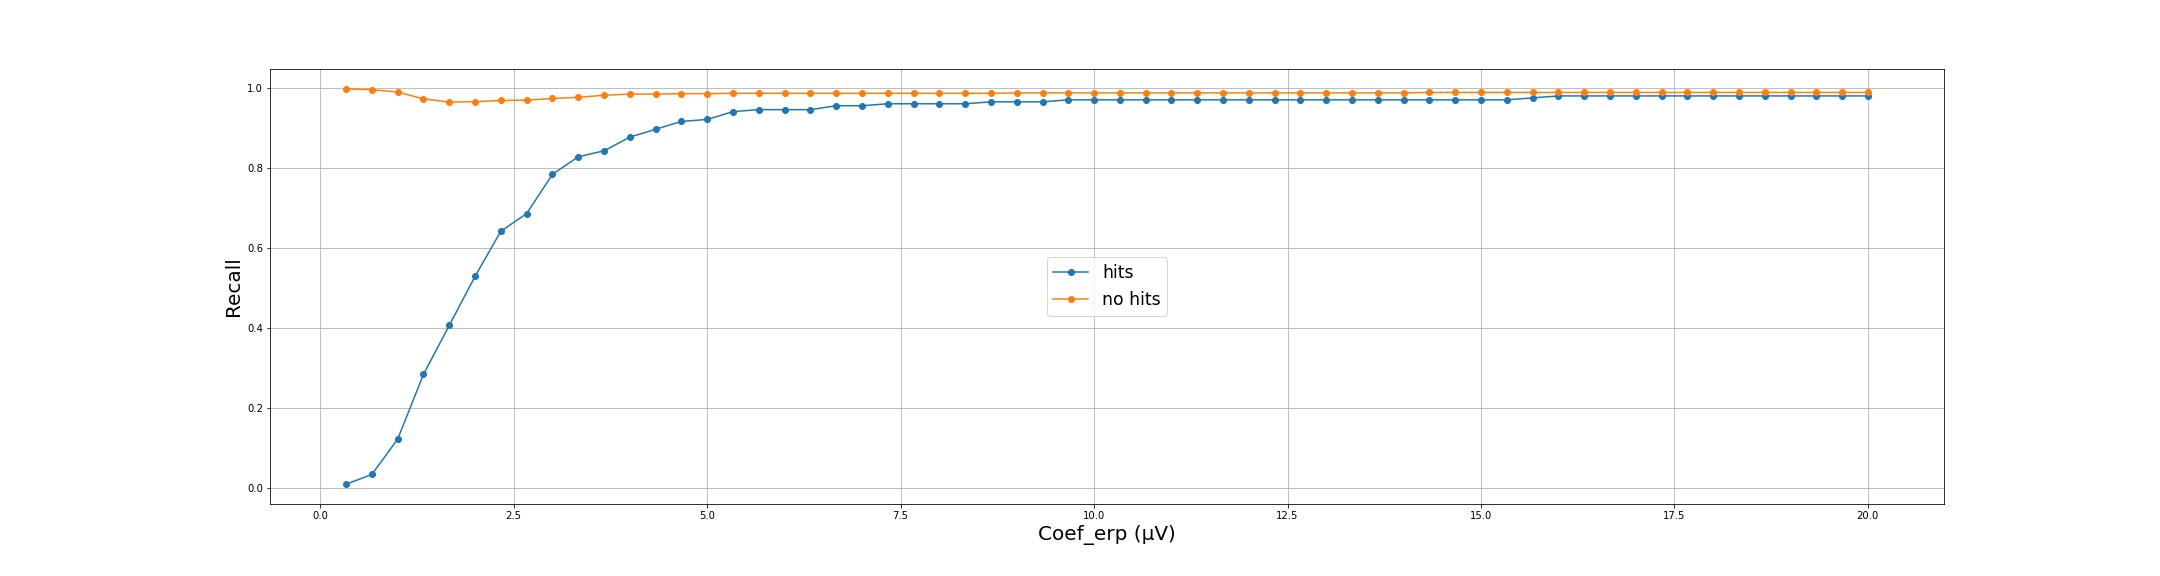
\includegraphics[scale=0.26]{02_Images/resultados_caso1_b_recall}
    \caption{Variación en uV para detectar el rendimiento en función de la métrica Recall.}
    \label{fig:resultados_caso1_b_recall}
\end{figure}  

El f1-score, dado por la combinación de las dos anteriores, confirma el resultado obtenido.

\begin{figure}[H]
    \raggedright
    %\includegraphics[width=15cm, height=8cm]
    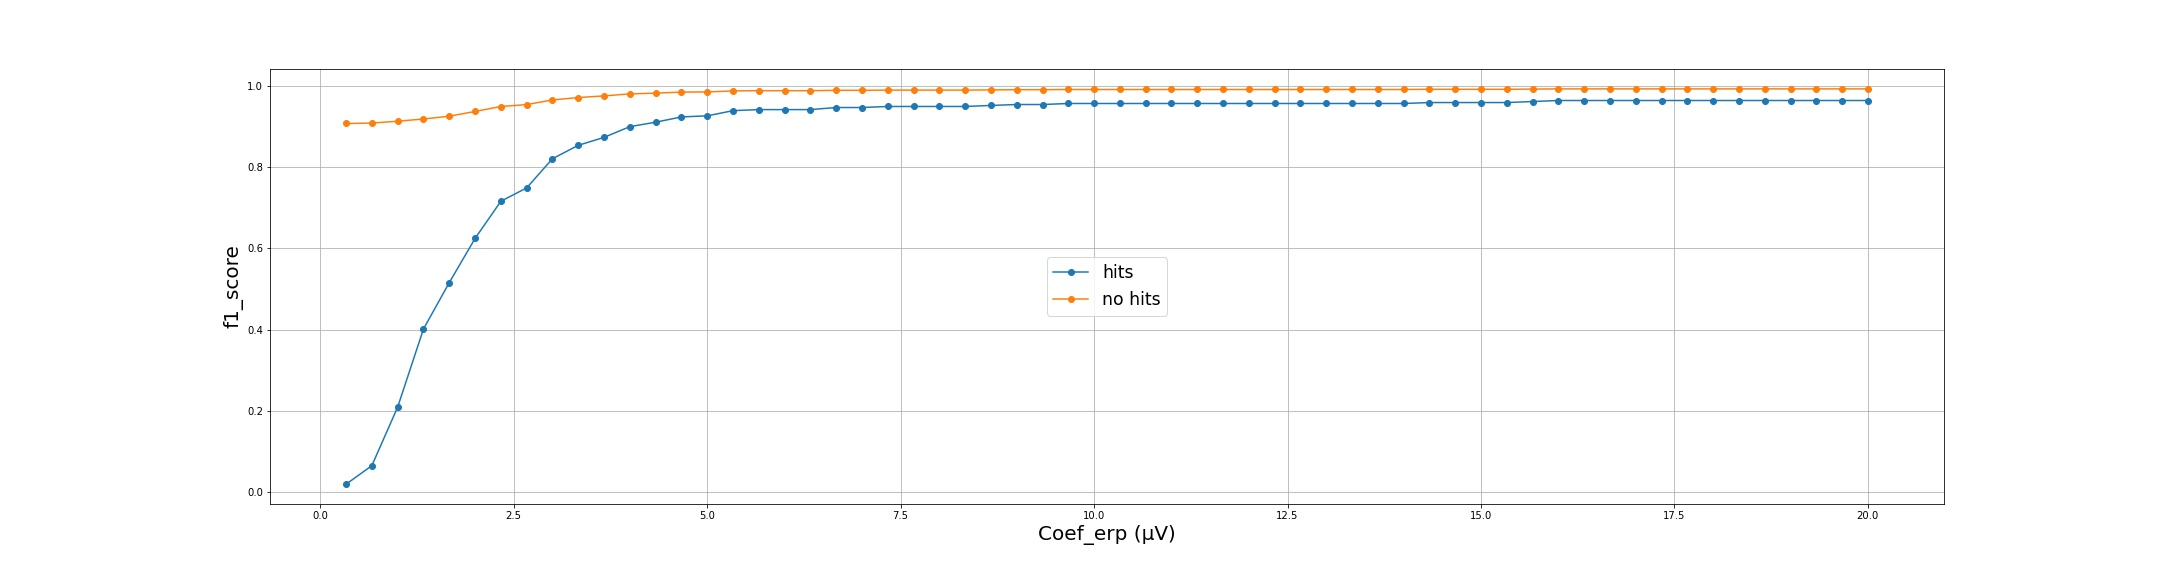
\includegraphics[scale=0.26]{02_Images/resultados_caso1_c_f1_score}
    \caption{Variación en uV para detectar el rendimiento en función de la métrica F1-score.}
    \label{fig:resultados_caso1_c_f1_score}
\end{figure}

\subsection{Variación en el tiempo.}
Misma metodología que el punto 9.1: Se generaron distintos vectores de distintos tamaños, con variaciones enteras y decimales, que permitieron genera desfase en el tiempo, cuya unidad es muestras. Las métricas arrojan que, \textbf{para alteraciones en el tiempo (muestras)}, no necesariamente ocurren mejoras en el rendimiento, ni tampoco comportamientos similares entre disparos hit/nohit. Es importante tenerlo en cuenta, ya que, es el total de la predicción la que impacta en el resultado. El desfase de las ondas modifica de manera directa y con altos márgenes en la predicción del algoritmo.
La métrica de precisión nos muestra relativa estabilidad en los nohits, mientras que en los hits ocurren variaciones que modifican notoriamente el resultado. 

\begin{figure}[H]
    \raggedright
    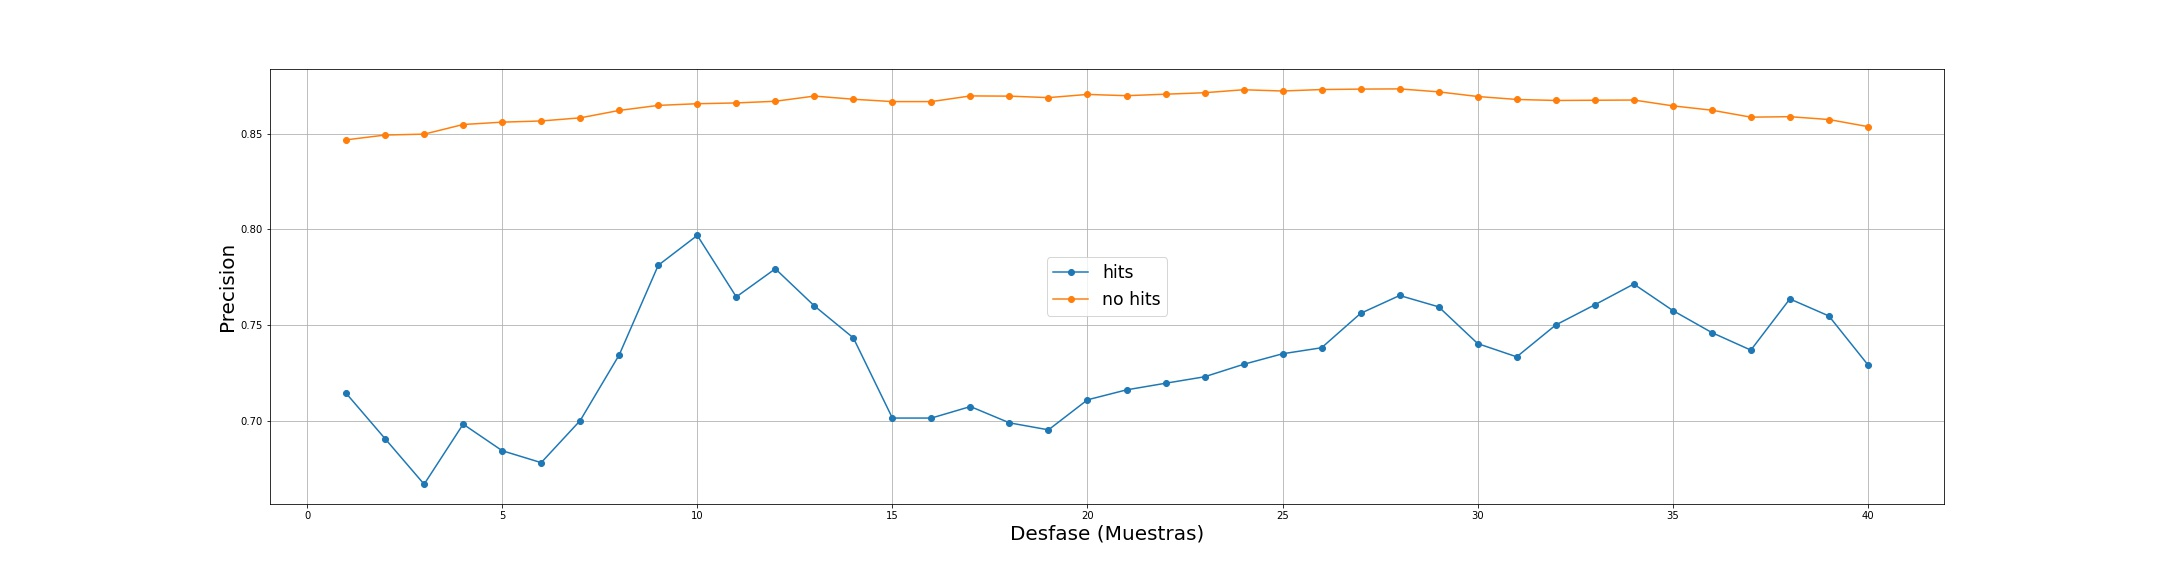
\includegraphics[scale=0.26]{02_Images/resultados_caso2_a_precision}
    \caption{Variación en cantidad de muestras para detectar el rendimiento en función de la métrica Presición.}
    \label{fig:resultados_caso2_a_precision}
\end{figure} \\

La proporción de resultados positivos que fueron identificados como tal, muestran en los hits un bajo rendimiento, afectando el resultado en conjunto.

\begin{figure}[H]
   \raggedright
    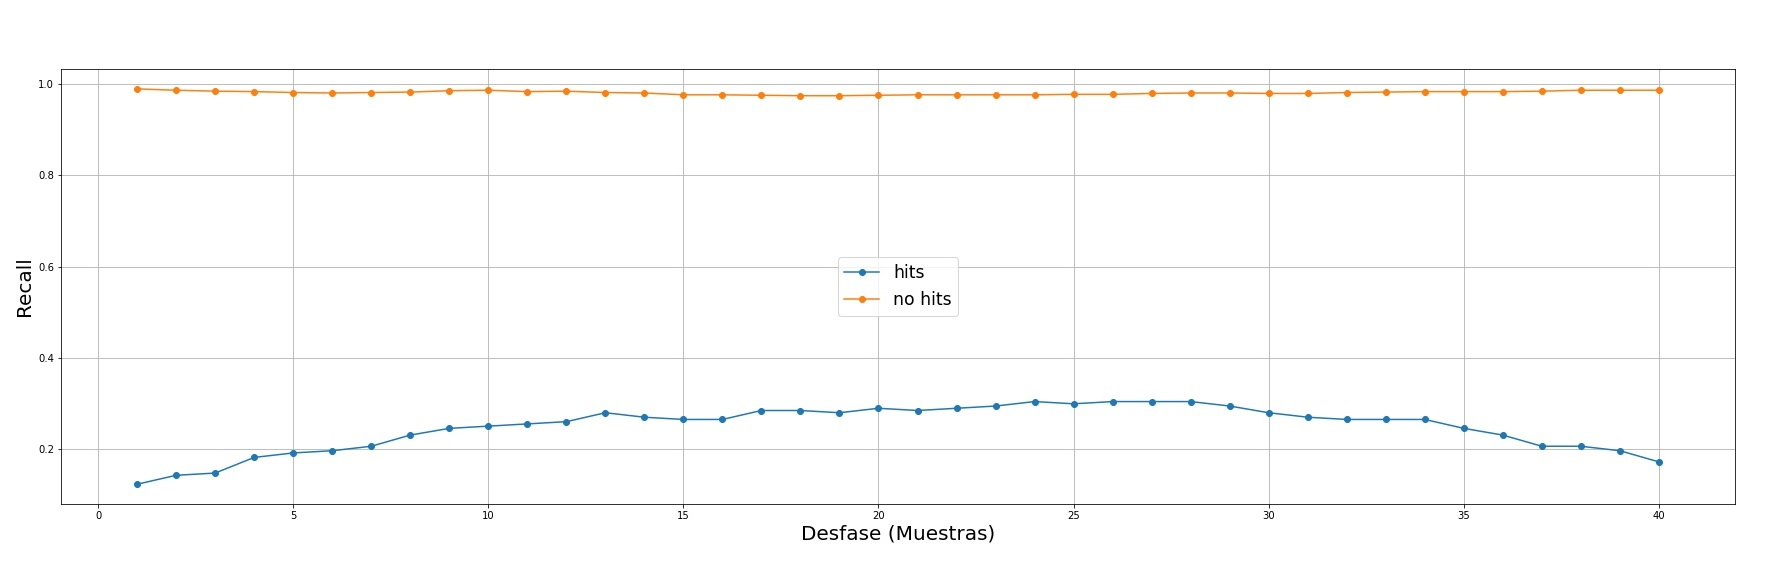
\includegraphics[scale=0.26]{02_Images/resultados_caso2_b_recall}
     \caption{Variación en cantidad de muestras para detectar el rendimiento en función de la métrica Recall.}
    \label{fig:resultados_caso2_b_recall}
\end{figure} \\

La combinación de las dos anteriores, compactado en la métrica mostrada en la siguiente gráfica, prácticamente replica el comportamiento de la métrica  \textit{recall}.

\begin{figure}[H]
    \raggedright
    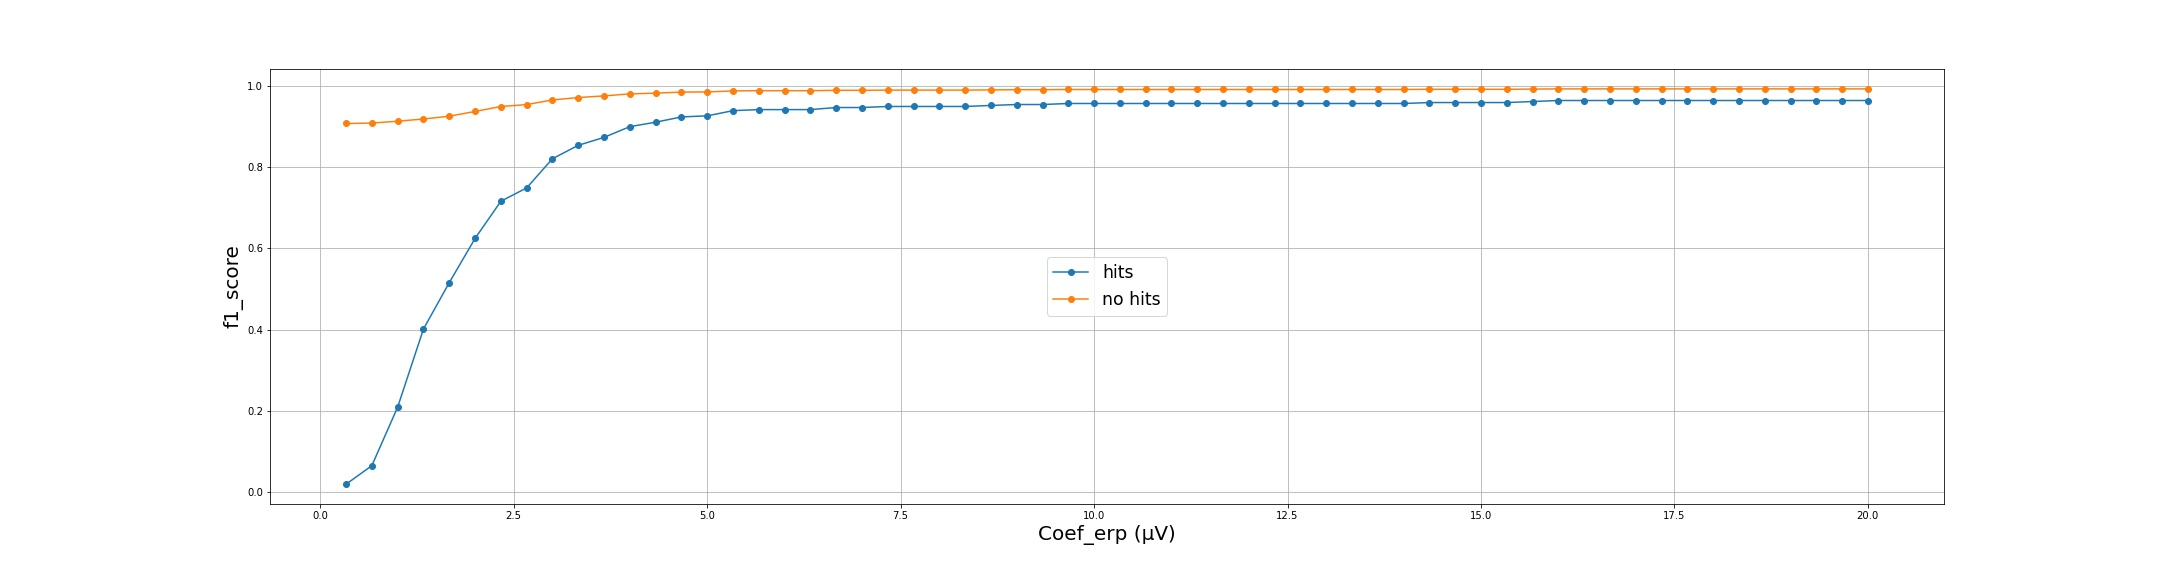
\includegraphics[scale=0.26]{02_Images/resultados_caso1_c_f1_score}
     \caption{Variación en cantidad de muestras para detectar el rendimiento en función de la métrica F1-Score.}
    \label{fig:resultados_caso1_c_f1_score}
\end{figure}

Los tres códigos trabajados son: 

\verb|a_Lag&DrugSignal_v6_CASO1.ipynb|,\\ \verb|a_Lag&DrugSignal_v6_CASO2.ipynb| y \\ \verb|a_Lag&DrugSignal_v6_CASO3.ipynb|. 

Se pueden encontrar en: \href{https://github.com/alexchavez1980/repo_tesis}{repositorio en GitHub}.

%\par\vspace*{\fill} % Moves keywords to the bottom of the page
%\textbf{\textit{Keywords --}} hardship, engineering, tired, verytired % Add you all the keywords associated with your thesis here

\biblio % Needed for referencing to working when compiling individual subfiles - Do not remove
\end{document}